% !TeX root =./main.tex
% !TeX spellcheck = en_US

Due to the global economic expansion of several industries and the dynamics of digitalization, the transport sector has been gaining massive momentum for years. Since 2010 global freight continuously increases with forecasts predicting growth rates of 3.2 \% until 2050 \cite{figura2020preferences, InternationalTransportForum}. Various transportation modes, including rail, maritime, air and road cargo are available to cope with this rapid international developments and to satisfy upcoming transport needs. At this point, road transportation is expected to be highly relevant due to its dominanting role for domestic transportation, with almost 80 \% of the total volume of goods being carried by trucks in the European Union \cite{Eurostat}. The increase in demand also holds true for the transportation of superheay and extra-large goods, refered to as oversize and heavy weight cargoes (OHC) in the rest of the article. OHC is typically associated with the transportation of bulky and overweight goods that require special planning and execuation on the road. In comparison with traditional freight transportation, OHC needs... In this paper we focus on the transportation of overweight goods which length is not necessarily the restricting parameter >  Planning of OHC transports takes usually several critical stages, where certain technical, administrative and organizational requirements have to be fulfilled. This is essence to ensure certain safety standards because OHC transports are in general beyond traditional road and therefore need to be planned in great detail. Planning of OHC and corresponding routes involves several stakeholders including private transport companies, governmental institutions and statics offices. Of course, in-detail planning is highly dependent on national standards but on a more general level the entire process involves the evaluation of multiple criteria related to restrictions on the physical characteristics of the road, road turning radius, total length of the route, demand for installation of transshipment sites or obstacles due to legal requirements. One of the most safety relevant attributes is the maximum bridge carrying capacity. Incidents of recent years underline the importance of detailed route planning of OHC to avoid long-term overtreatments of bridge statics, that potentially results in bridge collapse, as it was the case in Genova.

Over-weight load, i.e., vehicles loaded with more than 11 tons per axle,
are even harder to plan then over-size load. Over-sized load is limited
by road turning radius, transportation corridor width and road-side obstacles, such as traffic lights, power lines. Hence planning is dominated these local characteristics
and in-person inspection of the suggest route.

In contrast to that, the planning process for over-weight includes the consultation
of an civil engineer who must determine the allowable weight and speed to pass
complex building structures such as bridges.
This time consuming process must be repeated once the intended route is determined infeasible or changes for any other reason.
In an attempt to relieve some of this cumbersome workload from civil engineers,
we propose an mathematical optimization approach.
This labour intense planning procedure is described in
\citet{Osegueda.1999}.

To this end, a mathematical model determines the optimal path between two
points within the road network while respecting the bridge capacity constraints.
This serves as an \textit{decision support system} for civil engineers.
Ultimately,  each route must be must be approved by a civil engineer  in terms of
bridge capacities and other structural limitations.

Under the assumption that the model generates feasible routes,
we conduct a study that compares several (possibly conflicting) objectives.
Therefore, we consider different types of vehicles and different loads.

Possible objective are:
\begin{itemize}
  \item Shortest Path (classic).

  \item Minimal wear of infrastructure. Reducing the wear induced by over-weight transports
  minimizes maintenance costs, extends lifetime of the building structures, and
  improves safety (Genoa bridge collapse in 2018).

  \item Minimize the number of different road operators and municipalities the path
  traverses. In that sense, the process of getting official approval of the
  path should be simplified.
\end{itemize}

\begin{itemize}
\item Morandi Bridge Colapse

\cite{Morgese.2020}
\cite{MorandiNYTimes}


\item Commercial Solutions

\item HERE
\url{https://www.here.com/}
\item PRISMA
\url{https://www.prisma-solutions.com/}

\item Bentley Superload Routing
\url{https://www.bentley.com/en/products/product-line/asset-performance/superload-routing}



<<<<<<< HEAD:introduction.tex
\section{Matrix Representation of the Road Network}

For now, we consider the \textit{higher level road network} in Carinthia,
i.e., \textit{A}, \textit{S}, \textit{L}, \textit{B}, in form of a matrix.
The vertices of the matrix are the crossing points of the roads, while
the road section connecting those points form the edges of the matrix.
For each edge, we have the distance between the vertices and the length of the bridges along the segment and the capacity constraints (and the lowest encountered bridge capacity) for each edge.
This way, we can answer various questions concerning transports between those vertices.


=======
\item Road Network

We consider the higher level road network, i.e., A, S, L, B.
and we vertices of the matrix crossing points of the roads.
the edges are the road section between those points, for which we
consider the distance the length of the bridges and their capacity constraints (and the lowest encountered bridge capacity).
This way we can, answer questions concerning transports between those vertices.
\end{itemize}
>>>>>>> 8b8cbbbb4f65900ab49db8718d6c866383a01b00:sec1_Introduction.tex

\begin{figure}
 \centering
  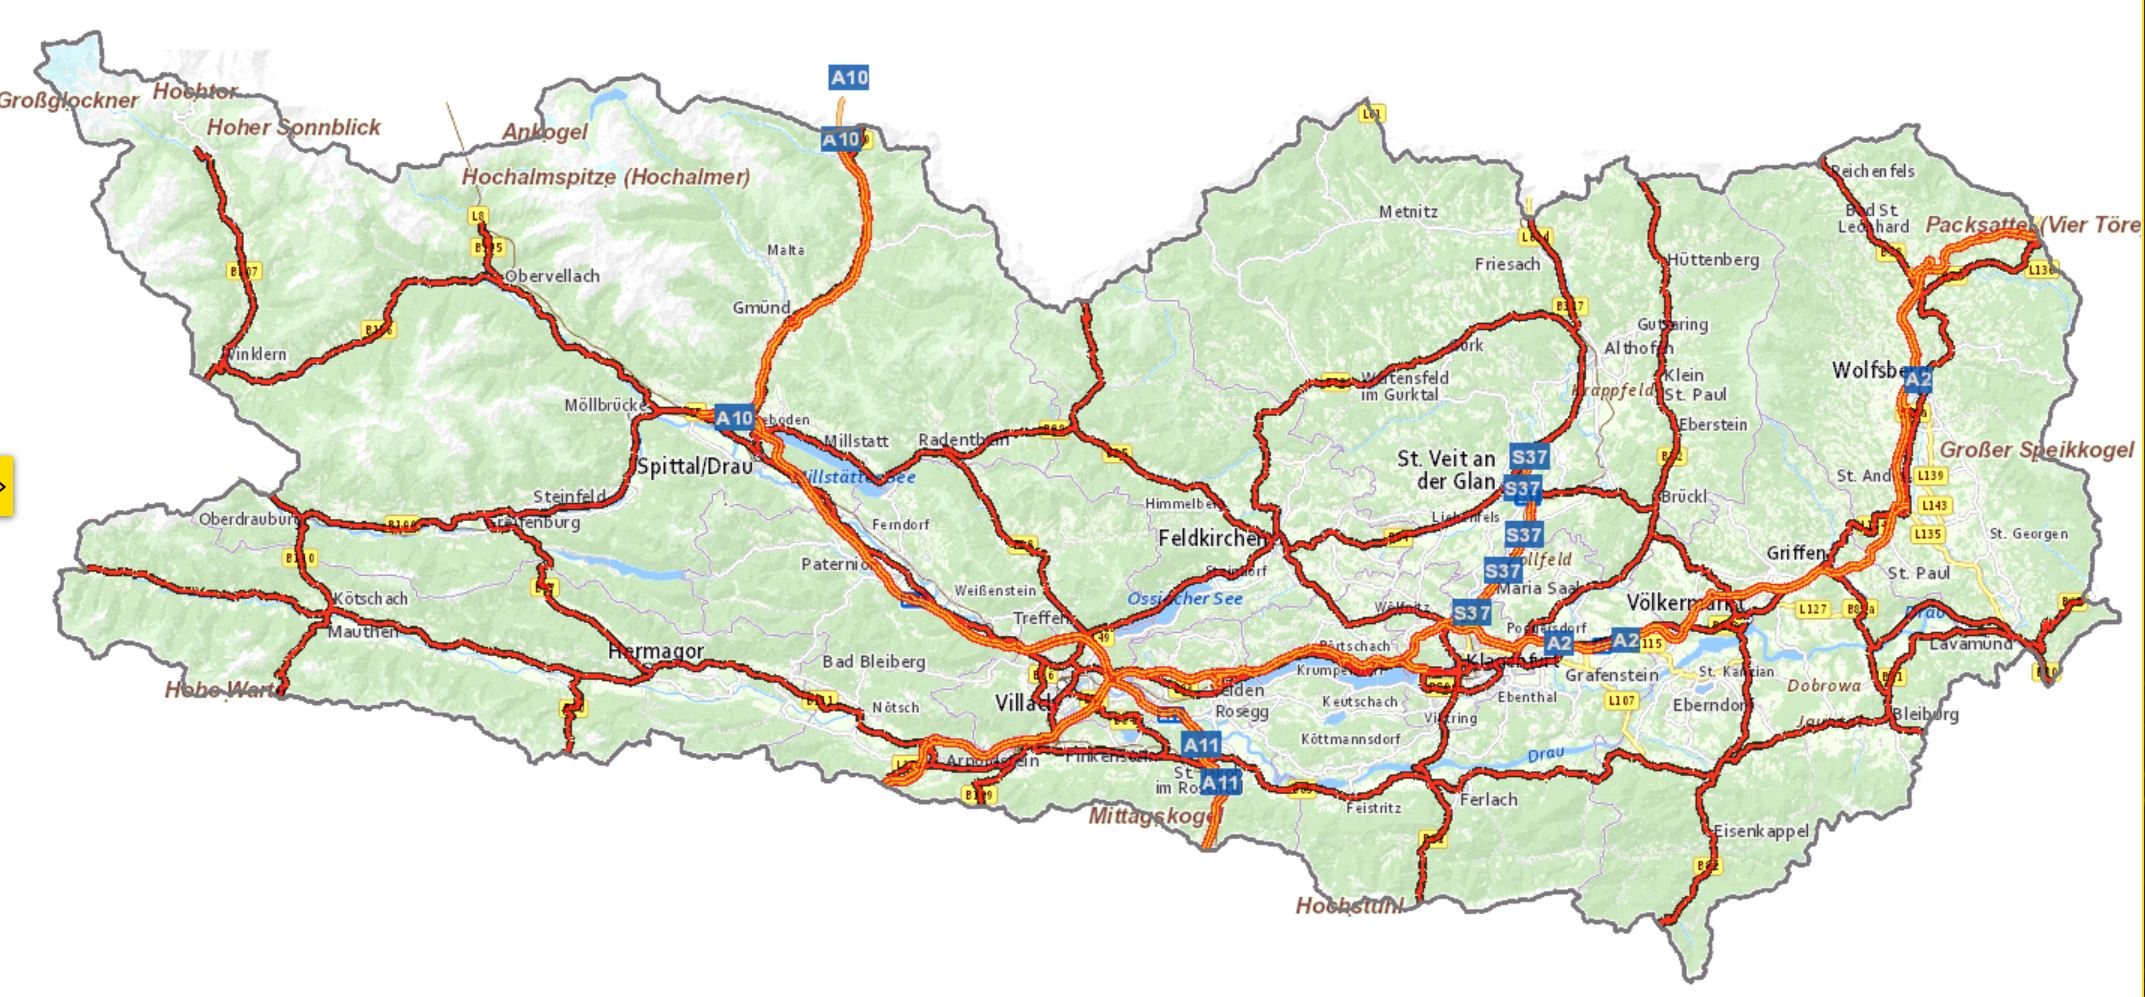
\includegraphics[width=0.9\textwidth]{map.jpg}
  \caption{Overview of the higher level road network in Carinthia.}
  \label{fig:higher level}
\end{figure}
